\section{Causal Framework for Discovering Heritability in Connectomes} 
\subsection{Heritability in Twin Datasets}
We focus on demonstrating the presence of heritability for structural connectomes in a twin neuroimaging study (see Figure \ref{fig:framework} for an overview). Figure \ref{fig:dag} illustrates a directed acyclic graph (DAG) representing a twin study, where measurements are obtained from individuals across multiple families. In the DAG, the directionality of arrows (e.g. $Z\rightarrow Y$)  indicates a potential causal influence of variable $Z$ on variable $Y$. Ideally, we aim to estimate the causal effect of genetic variation on structural connectome variation while controlling for all possible covariates, observed or unobserved. However, a key limitation is that estimating this pure causal effect is infeasible in practice, as it requires knowledge of both measured and unmeasured confounders.

Given the data available from twin neuroimaging studies, what models can help us provide evidence of heritability?
\begin{enumerate}
    \item \textbf{Associational Heritability:} The simplest model examines whether the genome is associated with connectomes. However, in real studies, both genome and connectomes are often influenced by other covariates. This makes estimated associational effects potentially unreliable, as they may conflate true genetic effects with those of correlated factors. For instance, if brain size relates to both genetics and structural connectomes, we cannot easily distinguish whether observed associations are due to genetics or neuroanatomy.
    \item \textbf{Conditional Heritability:} This model addresses the limitations of associational heritability. It asks whether differences in the outcome (structural connectomes) are associated with differences in genetic exposure, after conditioning on measured covariates. Observing such differences strengthens the argument for causal genetic influence.
\end{enumerate}

Conditional heritability can be considered equivalent to causal heritability under a sufficient condition: the strong ignorability assumption \cite{rosenbaum1983central}.  In twin studies, a simplifying assumption often made is the "equal environment assumption", that monozygotic (MZ) and dizygotic (DZ) twins share environmental factors to a similar degree by virtue of their study design. Additionally, in non-twin siblings, some overlap in covariate distributions is likely (e.g., if siblings share a household). Assuming that other experimental design considerations ensure overlap in covariates such as age, we can posit that neuroanatomy, sex, and age close all possible non-causal pathways that can create spurious correlations (e.g. close potential backdoor paths). If these conditions hold, the conditional heritability in our study can be interpreted as causal. 

% The genome that an individual inherits from his or her parents is the exposure, and the connectomes are the outcomes. We seek to estimate the causal estimand, which is the causal effect of the genome on the connectome. Both measured and unmeasured covariates can introduce confounding biases that affect both the exposure and the outcome. Unmeasured variables that affect the genome, such as race, fall under the category of \textbf{Nature}; unmeasured variables specific to life experiences, including both shared and unshared environmental influences, that affect the connectomes are classified as \textbf{Nurture}. Measured covariates, such as \textbf{Neuroanatomy}, \textbf{Sex}, and \textbf{Age}, also have an impact on the connectomes. 

\begin{figure}
\centering
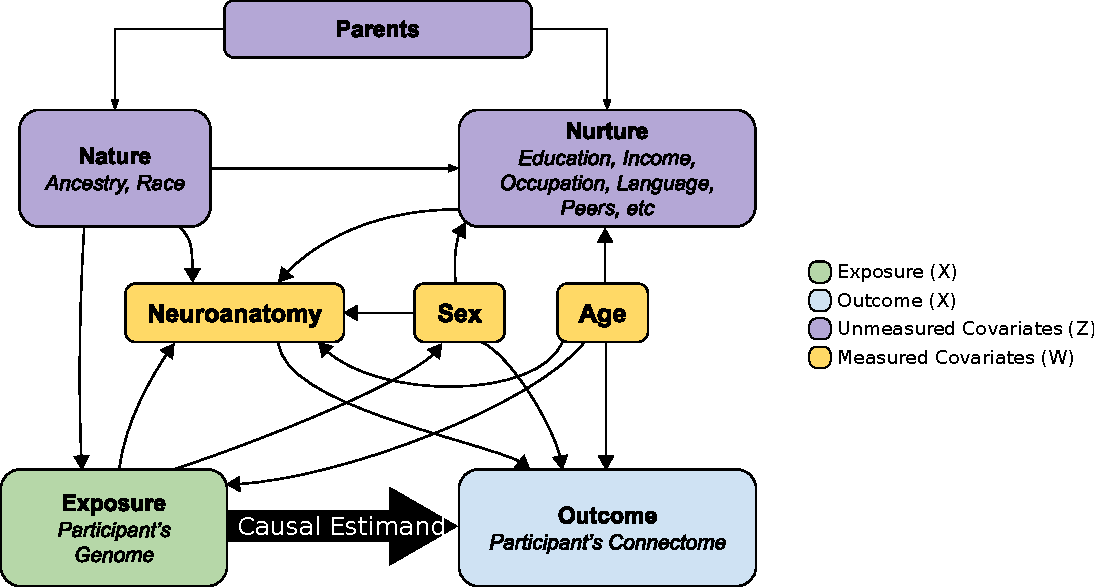
\includegraphics[width=0.8\linewidth]{figures/herit/dag.pdf}
\caption
[Causal Graph of Study Covariates.]
{\textbf{Causal Graph of Study Covariates.} Causal directed acyclic graph (DAG) presents a visual representation of the potential relationships between the genome and connectome, in the context of a twin study. The descriptions depict the various attributes that may be considered as exposures, outcomes, and covariates in such a study. In the absence of confounding, associational effects can be considered as causal effects. However, conditional effects can only be considered as causal when the covariates measured are sufficient to close all backdoor paths.}
\label{fig:dag}
\end{figure}

% The first step in \dcorr\ and \cdcorr\ is to compute the distance matrices, which encode the distances between all pairs of observations. Figure \ref{fig:framework} \textit{(center right)} shows examples of connectome and genome distance matrices. However, computing distances between connectomes is not straightforward because connectomes are high-dimensional and non-Euclidean data. In the following section, we present models and methods of computing distances between a pair of connectomes. 

\subsection{Twin Dataset for Discovering Connectomic Heritability}
We used an open access human brain diffusion (dMRI) and structural magnetic resonance imaging (sMRI) data set from the Human Connectome Project (HCP) Young Adult study, acquired by Washington University in St. Louis (WUSTL) and the University of Minnesota (Minn) \cite{hcp1, hcp2}. Out of the 1206 participants, a total of 1024 participant brain images were processed. Families with only one subject were discarded, and half-siblings were discarded. The data set includes 322 ($196$ females; ages $22-36$ years old, mean = $29.6$ and SD = $3.3$) monozygotic twins, $212$ ($125$ females; ages $22-36$ years old, mean = $28.6$ and SD = $3.4$) dizygotic twins, and $490$ ($237$ females; ages $22-37$ years old, mean = $28.3$ and SD = $3.9$) non-twin siblings. Structural connectomes were derived based on various parcellations. See \ref{sec:network_construction} for more details on network construction. Figure \ref{fig:data} shows visualizations of the average connectome and the difference in two most different subjects for the Desikan parcellation. 

\begin{figure}
    \centering
    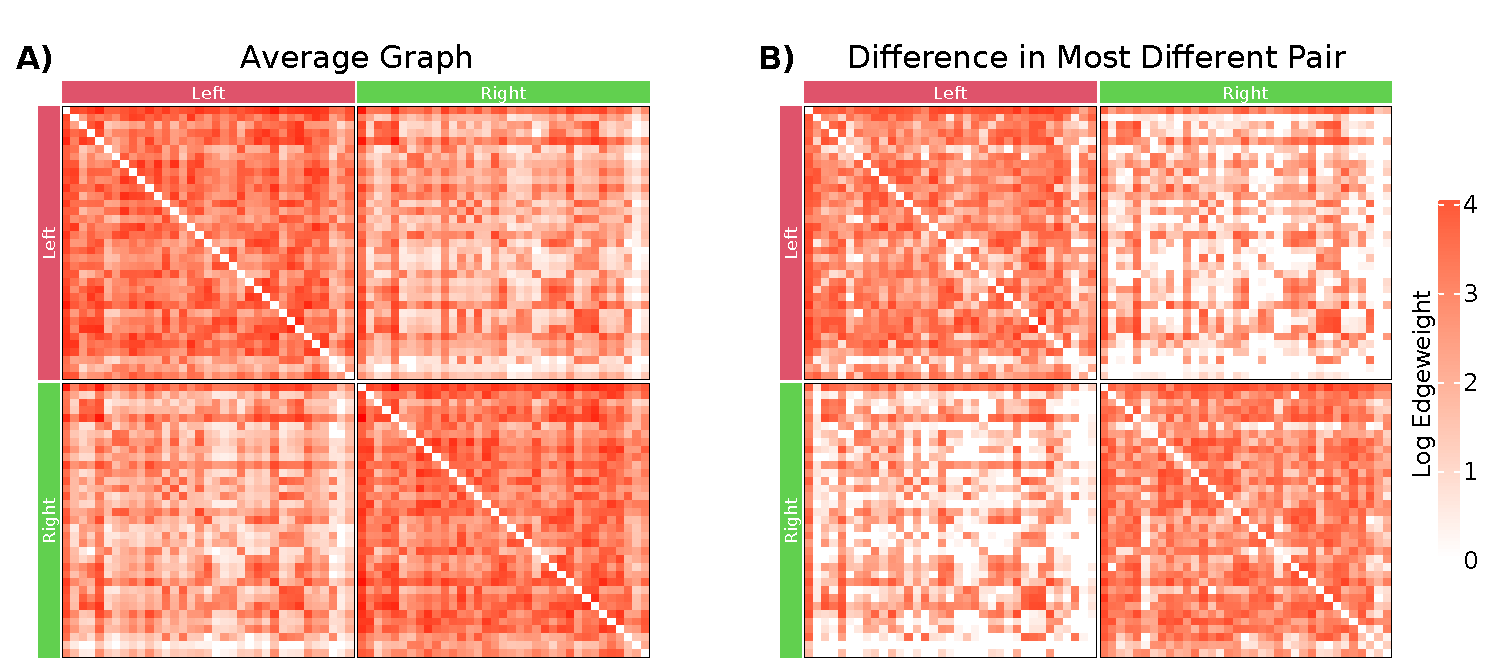
\includegraphics[width=\linewidth]{figures/herit/3-composite.pdf}
    \caption
    [Visualization of connectomes as adjacency matrices using the projected Desikan parcellation with hemispheric labels.]
    {\textbf{Visualization of connectomes as adjacency matrices using the projected Desikan parcellation with hemispheric labels.}  The projected Deskian parcellation was chosen for visualization purposes due to the low number of vertices ($n=70$). 
    \textbf{(A)} Average connectome of all subjects with log-transformed edge weights. 
    \textbf{(B)} Absolute difference of connectomes from the most different pair of subjects with log-transformed edge weights.}
    \label{fig:data}
\end{figure}

\subsection{Illustration of the Value of Statistical Models for Connectomes} \label{sec:heritability_models}
% Sentence about why statistical models for networks
% Dont mention rdpg, but a model where region has an latent vector
% We can estimate these vectors - mention methods for details
% Given these estimates for a pair of connectomes, we have three ways to compute differences between them - mention methods for mathematical details
% mention the three 

1. Networks inherently contain dependencies 
Networks inherently 
(refer to Section \ref{sec:statistical-models} for more details).
The random dot product graph ($\rdpg$) model provides a way to model weighted networks and compute differences between them using statistically principled procedures \cite{Young_Scheinerman_2007, sussman2012consistent, tang2017, tang2017nonparametric}. In this model, a vertex is a region-of-interest (ROI) in the brain, which is represented as a low-dimensional vector called a latent position. The probability of one ROI connecting to another is determined by the dot product of the corresponding latent positions. In other words, a matrix containing the latent positions of all ROIs is a representation of the underlying distribution of the connectome. Given these representations, we propose three different models for computing distances between connectomes (see Section \ref{sec:method-connectome-models} for more details):
\begin{enumerate}[leftmargin=*]
    \item \textbf{Exact model}: This model measures all differences between latent positions, with differences in the latent positions implying differences in the connectomes themselves. Consequently, a hypothesis test based on an exact model aims to test whether there is a correlation between the actual differences in connectomes and the differences in the genomes. 
    \item \textbf{Global model}: This model examines whether the latent positions of one connectome are a scaled version of the other. For example, if the number of edges in male connectomes are consistently larger than those in females, we have no way of differentiating whether significant findings from the exact model are a result of differences in scaling or differences in the fundamental structure of the connectomes themselves. Thus, hypothesis tests based on global model test whether differences in connectomes after adjusting for scaling differences correlate with differences in genomes. The global model assumes that the scaling factor is the same across all regions, meaning that any differences in scaling are not region-specific.
    \item \textbf{Vertex model}: This model is similar to the global model, but it allows for each vertex to be scaled differently. The idea behind this approach is that some vertices may have a greater impact on the overall network than others, so scaling them differently can provide a more accurate representation of the network. Consider the examples of how brain regions connect with each other. Regions in the same hemisphere are more likely to be connected than across hemispheres. Even within the same hemisphere, different regions may have distinct preferences for forming connections with other specific regions. Thus, hypothesis tests based on the vertex model aim to determine whether there are significant differences in connectomes after accounting for differences in vertex-wise scaling. 
    %Note that if the scaling is the same for all vertices, then the {vertex model} is equivalent to the {global model}.
\end{enumerate}

To demonstrate the differences in the connectome models, we simulated connectomes with various latent positions (Figure \ref{fig:simulations}). 
Columns I and II display four pairs of connectomes, each with specific latent position models. Rows (A-C) share the same underlying latent positions, while row (D) has different latent positions. When the connectome model can account for the differences in latent positions between the subjects, we observe a ``uniform'' structure in the differences, with no visible pattern. For the exact model (column III), distances increase as we move down the rows because it cannot account for any scaling, whether global or vertex-wise. We observe patterns in the differences, where red indicates edges in which subject $1$ tended to have more edges, while blue shows edges where subject $1$ tended to have fewer edges. For instance, for each simulation, when subject $1$ tended to have more edges (row B.I-II), we observe uniform red coloring in the differences (row B.III). Similarly, for the global model, we only see patterns in differences when the differences in latent positions are due to vertex scaling, as shown by the gradients of red and blue (C.IV and D.IV). The main takeaway is that any hypothesis tests based on these models can only make claims within the limits of their ability to explain the differences in the pairs of connectomes.

\begin{figure}
    \centering
    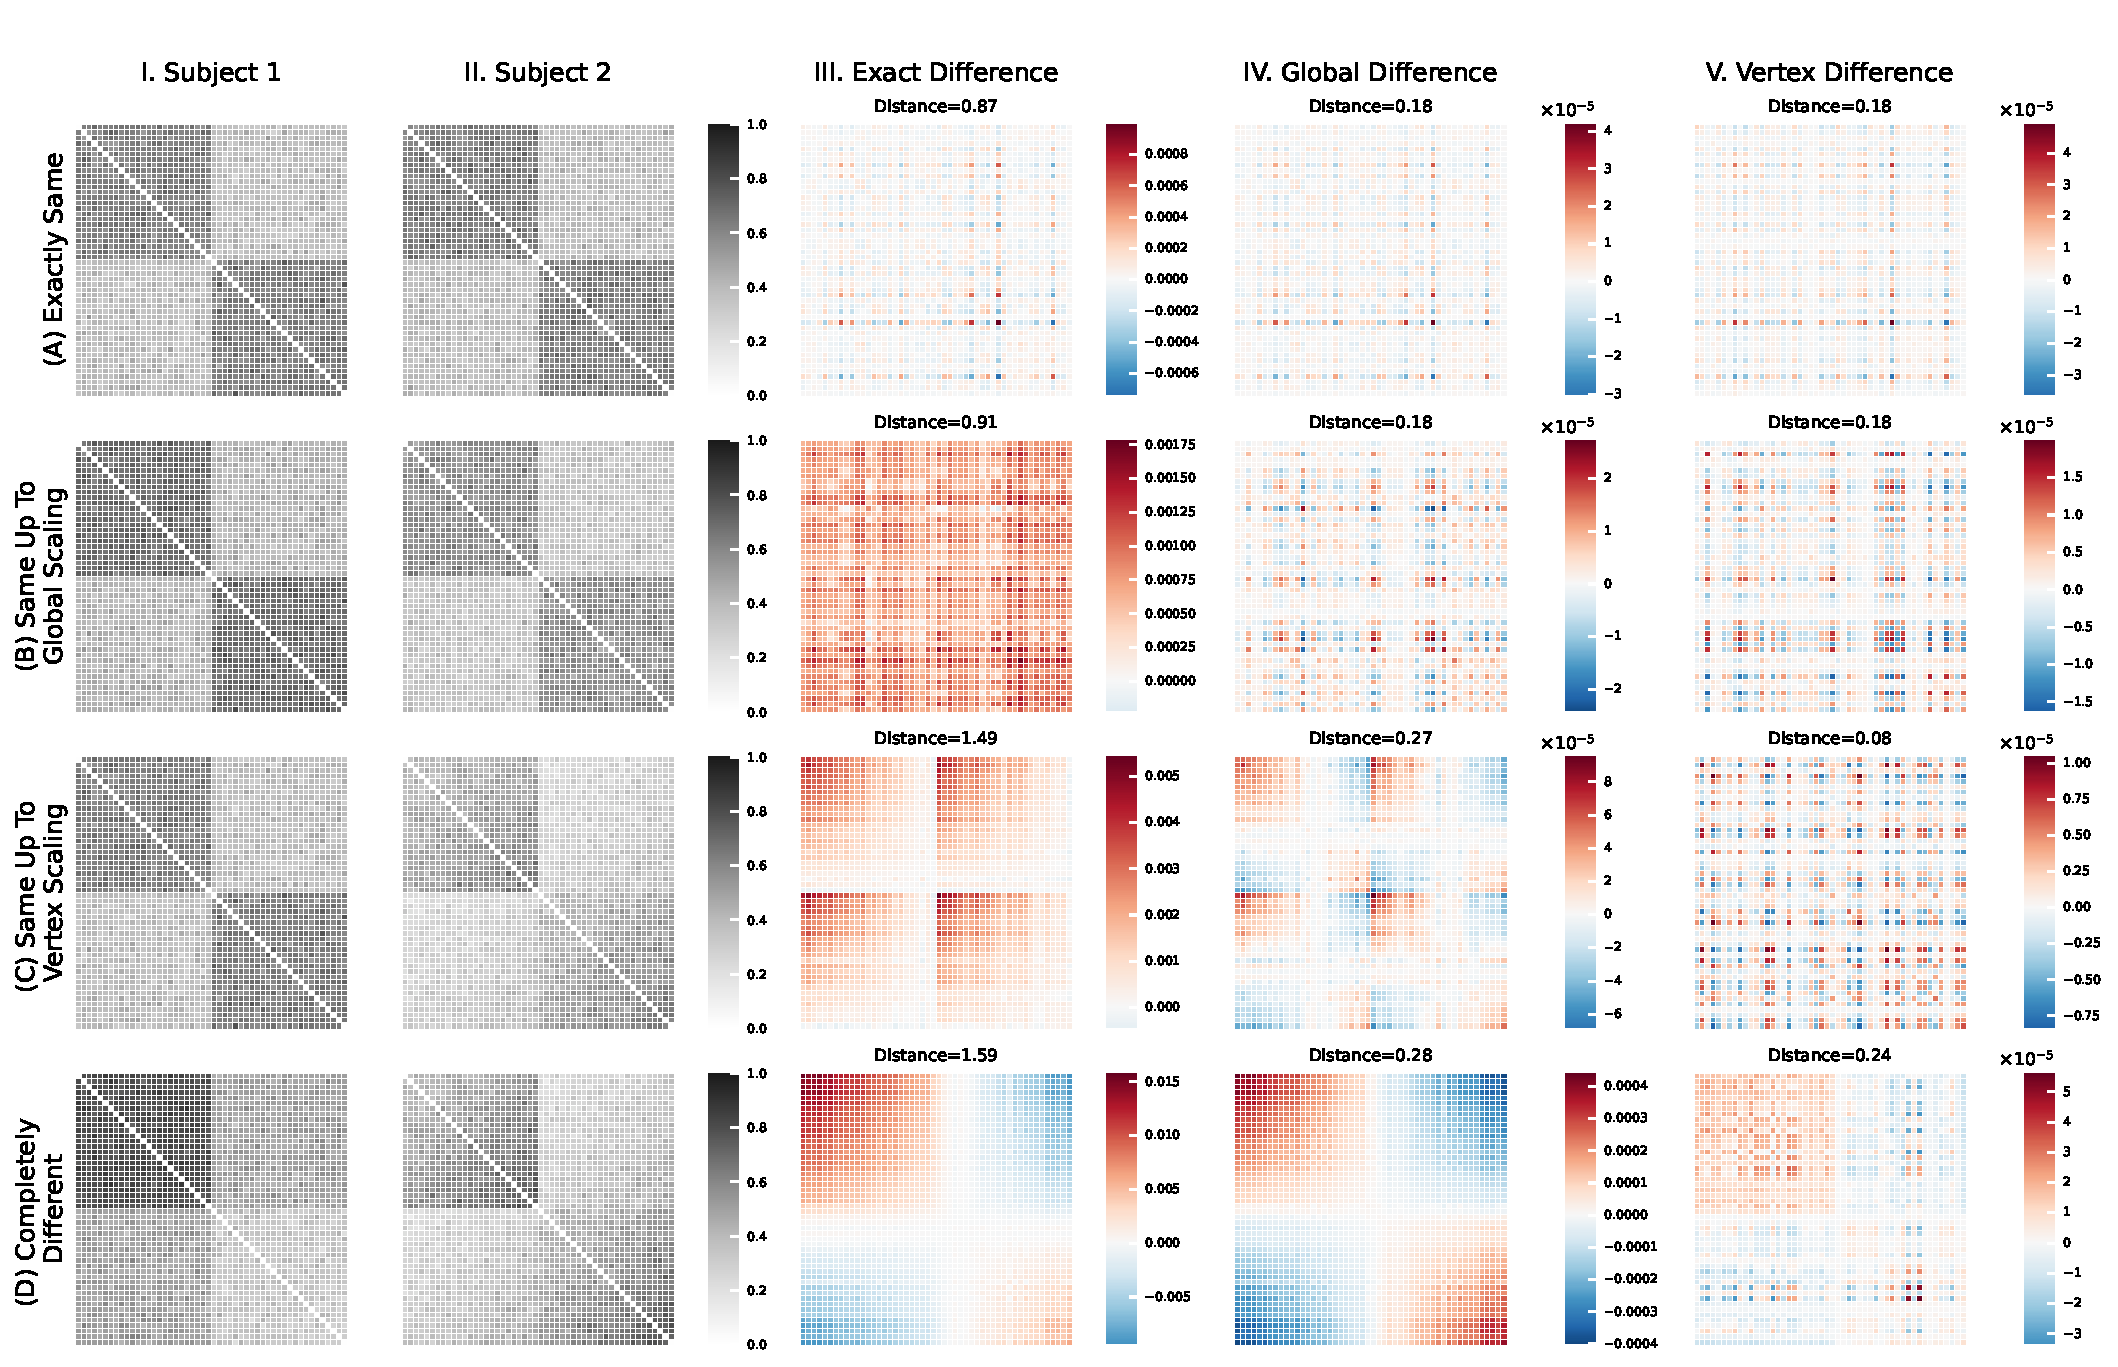
\includegraphics[width=\linewidth]{figures/herit/3-simulations.pdf}
    \caption
    [Simulations demonstrate the utility of connectome models.]
    {\textbf{Simulations demonstrate the utility of connectome models.} Connectomes with $50$ vertices were simulated $100$ times. Columns (I-II) display the average simulated connectomes, while columns {(III-V)} illustrate the differences in latent positions averaged over these simulations. In columns (III-V), red corresponds to when subject $1$ had more edges than subject $2$, while blue corresponds to when subject $1$ had fewer edges. Rows (A-D) correspond to various parameters used to generate the connectomes. Connectomes in rows (A-C) share the same latent positions, subject to scaling transformations, whereas connectomes in row (D) have distinct latent positions, conditional on scaling transformations. When the connectome models accurately represent the generative process, the difference matrix displays a "uniform" structure without discernible patterns (A.III-V, B.IV-V, C.V). However, when connectome models are not appropriate, patterns emerge, as indicated by the increased distance values (B.III, C.III-VI, D.III-V).
    For further technical details of these simulations, see Appendix \ref{sup:simulations}.}
    \label{fig:simulations}
\end{figure} 

\section{Results}

\subsection{Associational Tests for Connectomic Heritability} 

We begin the examination of heritability by first comparing connectomes from monozygotic and same-sex dizygotic twins. By limiting the comparison to these two groups, we minimized the impact of environmental factors (e.g. Nurture in Figure \ref{fig:dag}) on the connectomes and assessed the ability of connectomes to capture variations in the genome. Shared and non-shared environmental influences may arise due to differences in age or sex, which can lead to differences in upbringing or educational experiences. By controlling for such factors, we could reasonably attribute any differences in connectomes to variations in genomes rather than environmental factors. Moreover, if the differences in connectomes between monozygotic twins were ''smaller`` than those between dizygotic twins, it would suggest that connectomes can indeed capture variations in genomes. 
% This would support the idea that variations in the genome can manifest as differences in the connectomes, and thus provide insights into the genetic basis of brain connectivity. 

The distribution of connectome distances is shown in Figure \ref{fig:main-results}A.I-III by the blue and yellow rows, revealing that the medians of monozygotic twins ($N=127$) are smaller than those of same-sex dizygotic twins ($N=75$) for all three connectome models. To determine the significance of this difference, we perform a test for an associational effect using $\dcorr$, yielding $p <10^{-3}$ for all models (Figure \ref{fig:main-results}B.I). These results provide our first evidence for the heritability of connectomes. We then expanded our examination to include non-twin siblings and unrelated subjects (Figure \ref{fig:main-results}A.I-III green and red rows) and observed that the medians grow larger as the familial relationships grow distant. Based on these observations, we tested for associational heritability across all familial relationships, yielding p-values of $<1\times 10^{-3}$ for males and females under all three heritability models (Figure \ref{fig:main-results}B.II). All of these tests indicate a strong associational effect of the genome on connectomes.

\begin{figure}[htp]
\centering
\includegraphics[width=\linewidth]{figures/herit/Desikan-composite.pdf}
\caption
[Testing associational and causal effect of genome on connectomes and neuroanatomy.]
{\textbf{Testing associational and causal effect of genome on connectomes and neuroanatomy.}
\textbf{(A)} Each point represents the pairwise distance between pairs of participants; diamond markers represent the median distance, colors are familial relationships, and rows are sex. 
\textbf{(A.i-iii)} The median distances revealed that MZ twins exhibited smaller distances compared to DZ twins, siblings, and unrelated pairs, whereas the unrelated pairs showed larger distances. DZ twins displayed smaller distances compared to siblings and unrelated pairs, but larger than those of MZ twins. These findings provide qualitative evidence of heritability of connectomes. 
\textbf{(A.iv)} The median distances of neuroanatomy also show qualitative evidence of heritability. 
\textbf{(B)} Colors of heatmaps represent p-values, rows are gender groups, and columns are connectome models. (B.I-II) Associational test for connectome heritability. In (B.I), we only compare MZ and DZ twins, and the significance tests provide evidence of heritability as shown in (A.I-III). In (B.II), we conduct tests across all three familial relationships and observe significant effects, providing further evidence for connectomic heritability. In contrast, in (B.III), we observe significant effects for neuroanatomy, suggesting that the results in (B.I-II) may be confounded by an effect mediator. Subsequently, in (B.IV-V), we perform causal tests for connectome heritability. In (B.IV), we observe significant results only for the exact and global models, indicating that the connectomes remain heritable even after conditioning on the anatomical covariates, age, and sex. This suggests that the results in (B.I-II) cannot be entirely explained by neuroanatomy. The non-significant tests using the vertex model suggest that when we control for covariates and vertex-wise scaling, we can no longer detect heritability. In (B.V), we define a non-heritable subgraph as a collection of vertices that are not heritable by the causal test. We still observe several significant tests, suggesting heritability remains even after discarding vertices.
} 
\label{fig:main-results}
\end{figure}
 
\subsection{Associational Test for Neuroanatomic Heritability} \label{sec:neuroanatomy-dcorr}
Multiple studies have investigated the heritability of human brain anatomy \cite{blokland2012genetic, ge2016multidimensional, brouwer2014heritability, thompson2001genetic, lee2016partitioning, den2013heritability}. 
Structural MRI studies on adults have shown that genetic and environmental factors have a significant impact on brain properties such as volume, shape, and both cortical and subcortical structures.  This suggests that neuroanatomy could be an effect mediator (Figure \ref{fig:dag}).
 To assess if neuroanatomy could be a mediator, several features such as brain volume, axial diffusivity (AD), radial diffusivity (RD), and fractional anisotropy (FA) were computed for each region of the brain. Refer to Section \ref{methods:covariates} for more details. 

We used $\dcorr$~to test for the associational effect of the genome on anatomical covariates. This test assumes that if the covariates and genetics are independent, then brain anatomy is not heritable and has no effect on connectomes. Conversely, if the alternative is true, the associational effects of heritability of connectomes may be partially explained by the heritability of the anatomy itself, making the brain anatomy an effect mediator. Figure \ref{fig:main-results}A.IV illustrates that similar to connectome distances, the median distances increase as familial relationships become more distant. Furthermore, we find that the tests showed $p<10^{-3}$ for all three gender groups under all three connectome models (Figure \ref{fig:main-results}B.III). The significance suggest that the associational heritability of connectomes may partly be due to the effect of anatomy on connectomes. 

\subsection{Causal test for connectomic heritability}
\label{sec:conditional_dcorr}
To account for the dependence of neuroanatomy on genetics, we utilized conditional distance correlation ($\cdcorr$) to estimate the conditional effect of genome on connectomes (Eq. \ref{eq:conditional-hypothesis}). The covariate set also included age, which is a confounder. 
% If the null hypothesis result implies that similarities in brain connectivity are completely explained by similarities in brain anatomy and age, whereas a significant result suggests that the connectomes contain information on brain connectivity beyond anatomy and age, which is still heritable. 
Our results showed $p<10^{-2}$ for exact and global models, but showed $p>.1$ for the vertex model. This indicates that while connectomes are heritable and not entirely influenced by anatomy and age, there is no significant underlying structure beyond the vertex-wise scaling. This contrasts with the results shown in Figure \ref{fig:main-results}B.I-II, highlighting the importance of causal modeling in this study.

\subsection{Non-heritable Subgraphs are also Heritable} \label{sec:subgraphs}
In this section, we consider the possibility that heritability effects detected in Section \ref{sec:conditional_dcorr} are driven by a subset of vertices rather than the entire connectome. That is, it is possible that the connectivity of a subset of brain regions may be highly similar in twins but highly different in non-twin siblings or unrelated individuals. To investigate this, we test for causal heritability by examining the \textit{non-heritable subgraphs}, which are subgraphs induced by the vertices in which no heritable effect can be detected. See Section \ref{sec:cond-effect-vert} for more details on the hypothesis.

The outcomes presented in Figure \ref{fig:main-results}B.V display significant p-values for both the exact and global models across all genders, with only the exact model presenting significant p-values in males. These results suggest that for females, heritability can be fully accounted for by the heritable vertices, while in males, the non-heritable vertices still demonstrate heritability. Nevertheless, when controlling for scaling, the significance observed in the exact model for males is eliminated, indicating that differences in the scaling of the subgraphs explain the observed significance. These findings suggest the presence of an underlying structure in the non-heritable subgraph that cannot be detected at the level of individual vertices and highlights the necessity of statistical modeling of networks.